\documentclass[12pt,a4paper]{article}
\usepackage[utf8]{inputenc}
\usepackage{graphicx}
\graphicspath{ {images/}}
\begin{document}
\title{
Deliverable 1: Final Year Dissertation\\
\vspace{10mm}
Evolving a Learning Agent using Neuroevolution in the FightingICE Game Platform\\
\vspace{25mm}
}
\date{}
\author{Robert John Dunn\\
H00163867\\
BSc Honours in Computer Science\\
Heriot-Watt University\vspace{15mm}\\
Supervisor:\\
Dr Patricia A. Vargas\vspace{3mm}\\
Co-Supervisor:\\
Dr Fabrício Olivetti de França\vspace{3mm}\\
Second Reader:\\
Dr Mohamed Abdelshafy
}
\maketitle
\newpage
\vspace*{30mm}
\section*{Declaration}
I,  Robert Dunn confirm that this work submitted for assessment is my own and is expressed
in my own words. Any uses made within it of the works of other authors in any
form (e.g., ideas, equations, figures, text, tables, programs) are properly acknowledged
at any point of their use. A list of the references employed is included.\\
\\
Signed:\\
\\
Date: 
\newpage
\begin{abstract}
Neuroevolution is a popular technique for machine learning in which an artificial neural network is trained by an evolutionary algorithm. The technique takes inspiration from the evolution of the biological nervous system and is a popular approach for reinforcement learning problems. One way to demonstrate the effectiveness of neuroevolution is through artificial intelligence in games. This project aims to implement a learning agent in the FightingICE platform, a two-dimensional Java fighting game organised and maintained by Ritsumeikan University, Kyoto. The agent is designed to evolve through neuroevolution to improve its performance in the game, eventually becoming competitive versus a human opponent. By implementing a neuroevolution method in a simplistic environment, we hope to evaluate the effectiveness of neuroevolution as a method of machine learning and explore the potential of our agent's performance.
\end{abstract}
\newpage
\tableofcontents
\newpage
\section{Introduction}
Machine learning is a heavily researched field of artificial intelligence in which machines are given the ability to learn without being explicitly programmed. Various methods of machine learning exist which allow the machine to adapt itself in order to process new data. One of these methods is neuroevolution, which involves an artificial network being trained with an evolutionary algorithm to imitate the learning process.\\

The neuroevolution method is loosely based on the way the biological nervous system operates: with neurons communicating through axons, represented by nodes of the neural network with weighted connections. Neuroevolution is a form of reinforcement learning, which means a notion of reward is introduced and the machine attempts to maximise said reward. The wide application of reinforcement has given neuroevolution popularity in the fields of artificial life and evolutionary robotics. This notion of reward also allows the method to easily be applied to computer games since the reward is usually simple to measure, e.g. the hit-points of the player's character.\\

This project aims to implement a neuroevolution algorithm acting on a learning agent in the FightingICE game platform. FightingICE is a two-dimensional fighting game written in Java by Intelligent Computer Entertainment Lab, Japan. The platform allows easy implementation of artificial intelligence by sending delayed game information to the agent. Using neuroevolution we hope to evolve an agent to the point of being competitive versus a human opponent, though not unbeatable. The performance of the agent will be evaluated at various stages of the evolution in order to evaluate the effectiveness of our algorithm.\\

The next section of this dissertation is the literature review which discusses and evaluates relevant technical literature. Followed by requirements for the project identifying system requirements for the target system. Next, the evaluation strategy for the project is presented which details evaluation and analysis to be conducted. Finally an overview of management for the project which includes a timetable for the project, analysis of risks, and considerations of professional, legal, ethical and social issues.
\newpage
\section{Literature Review}
\subsection{Machine Learning}
\subsubsection{Learning Paradigms}
Learning is an essential human function in which we modify our behaviour tendency according to experiences, to become better when a similar situation occurs. In the study of machine learning, algorithms, computer applications, and systems, utilise learning to improve their performance at certain tasks. There are two main entities in the machine learning model, the teacher and the learner. The teacher contains the knowledge to perform a given task while the learner has to learn the knowledge the teacher holds. \cite{swarmann} There are three types of machine learning [pat]:
\begin{enumerate}
\item \emph{Supervised Learning}\\
A teacher provides the learner with a set of input and desired output pairs. The learner can then use these examples to improve its performance at the task.
\item \emph{Unsupervised/Self-organised Learning}\\
There is no teacher, so the learner learns based only on the stimuli received. A common application is finding patterns or grouping within data, using methods such as cluster analysis.
\item \emph{Reinforcement Learning}\\
The agent uses goal-directed learning where a notion of reward is introduced and the agent attempts to maximise this reward. There is no teacher for the agent and no explicit model of the environment.
\end{enumerate}

\subsubsection{Incremental Evolution}
When an agent is provided with a complex behaviour, it may have trouble evolving to perform at its potential. Using incremental evolution, the behaviour can be learnt incrementally with tasks gradually increasing in difficulty. This form of evolution proved effective in one implementation \cite{incre}. The agent's task was a prey capture task: the agent moves through the environment and must catch its prey before the set number of time-steps. With increasingly difficult tasks, the agent was able to rapidly improve its performance, and skip many potential generations of evolution.

\subsection{Neuroevolution}
\subsubsection{Fundamentals}
Neuroevolution is a popular biologically-inspired method of machine learning in which an artificial neural network is evolved using an evolutionary algorithm. The method has proved popular, especially in the fields of artificial life, evolutionary robotics and computer games. One reason for its popularity is the fact that neuroevolution is a form of reinforcement learning, which can be applied more generally than its counterpart, supervised learning. 

\subsubsection{Artificial Neural Networks}
Artificial neural networks model the way the brain solves problems with collections of neurons communicating through axons, represented with neurons with weighted connections. Neural networks have an associative (content-addressable) memory and can also implement parallel processing. They are often applied to pattern finding within data.

\subsubsection*{Topology}
The most basic version of an ANN (artificial neural network) is a perceptron. A perceptron is a simple machine which takes a variable number of input nodes which connect to a single output node. From the perceptron evolved the multi-layer feed forward network, which incorporates extra 'hidden' layers of neurons between the input and output. The more hidden layers there are and the more nodes in these layers, the more complex behaviour a network can experience. 

\newpage
\subsubsection*{Activation Function}  
In order to saturate neuron values to a usable range (usually -1 to 1), an activation function is used. The most basic version of this function is ?, where any values below zero will result in an activation of zero, and any values above zero in an activation of one. It is also possible to use more general, non-linear functions such as the tanh function, shown below.
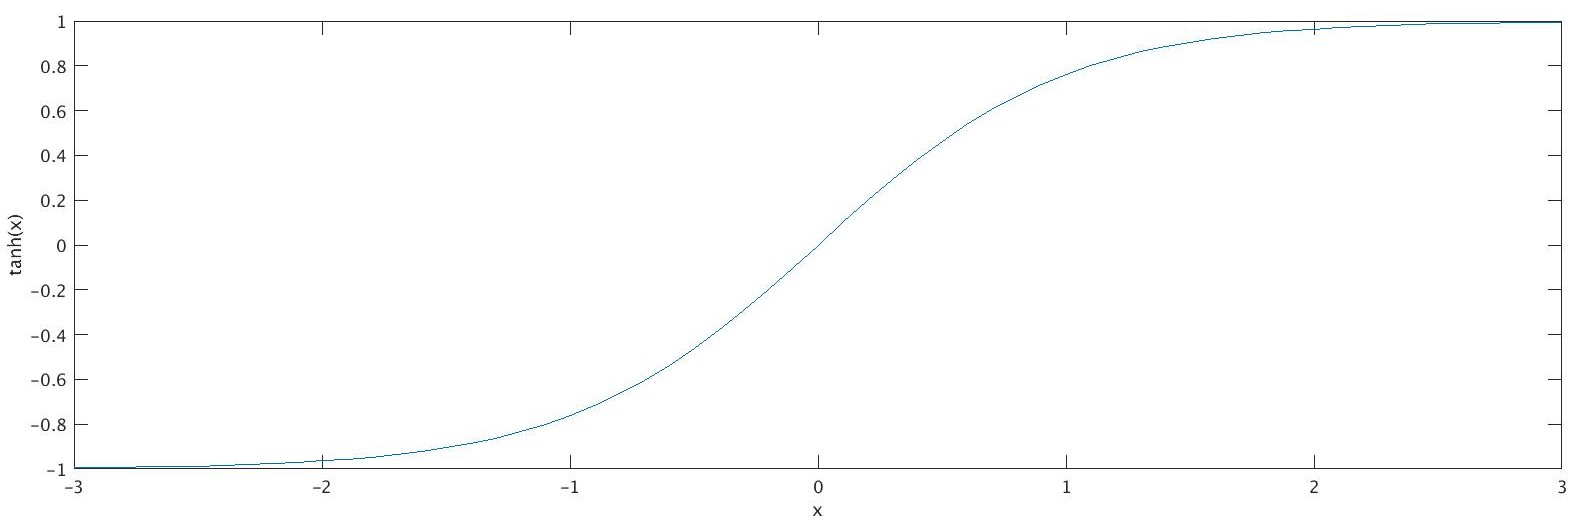
\includegraphics[width=\textwidth]{tanh}
Another possibility is to have neurons operate probabilistically.[add more]

\subsubsection*{NEAT (Neuroevolution of Augmenting Topologies)}
TO DO


\subsubsection{Genetic Algorithms}

\subsubsection{Neuroevolution in Games}
How neuroevolution can be used to evolve learning agents in games, usually agent is optimising some value e.g. HP. How fitness in games is evaluated, giving some examples. How neuroevolution fares compared to other learning algorithms. Present examples of projects implementing neuroevolution to learn.

\newpage
\subsection{FightingICE}
\subsubsection{Game Platform}
FightingICE is a Java based game platform organised and maintained by Intelligent Computer Entertainment Lab., Ritsumeikan University. The game is based in an arena where two fighters are competing versus each other, attempting to deplete the other's hit-points while preserving their own. The FightingICE platform was designed to allow easy development and evaluation of artificially agents in the game for research or hobby purposes. Once implemented, an agent receives information about the state of the game from the platform periodically, such as the opponent player's location and current energy levels. A delay is added to this game information in order to simulate the delay a human player would experience from reaction time.\\
\includegraphics[width=\textwidth]{fightingICE}

\subsubsection{Game Agents}
Agents in the game have two main attributes- hit-points and energy. There are four characters available in the game: Zen, Garnet, Lud, and Kfm. Each of these characters is capable of moving, performing attacks, and combing these attacks into deadly combos. 
Present information on the agents in the FightingICE game. The capabilities of the agents including which attack moves / movement commands they can do. Touch on fitness evaluation (how to win the game: keep enemy HP low and your HP high).\\


\subsubsection{Related Projects}
Discuss and reference relevant projects which have been completed using the FightingICE framework. Discuss what has been achieved in said projects and the potential further research that can be undertaken.

\newpage
\section{Requirements}
Functional:

FR-1 : The agent should be barely competitive versus a human opponent.

FR-2 : A neural network to control the agent's behaviour should be implemented.

FR-3 : An appropriate evolutionary algorithm to evolve the neural network (see FR-2) should be implemented.

FR-4 : The agent's performance versus a human opponent at various stages of evolution should be evaluated.

FR-5 : The agent should be coded in the Java FightingICE platform.\\

Non-functional:

NFR-1 : Incremental evolution could be utilised to skip some generations of evolution.

NFR-2 : Evolution of the neural network could be visualised.
\newpage
\section{Evaluation Strategy}
Evaluation of the agent's performance will be calculated through the character's hit-points attribute. In FightingICE, both players start at zero hit-points and connected attacks cause these hit-points to be reduced below zero. Once the game is finished, comparisons can be made between both player's hit-points to evaluate the performance of the agent.\\

Evaluation will consist of games played versus a human opponent at different stages of the agent's evolution. This will allow us to analyse how the agent's performance improves over time and in turn the effectiveness of neuroevolution.\\

[ADD MORE]

\newpage
\section{Project Management}

\section{References}

http://www.cs.utexas.edu/users/nn/downloads/papers/gomez.ijcai99.pdf

https://arxiv.org/abs/1608.02971

https://arxiv.org/abs/1604.00644

https://arxiv.org/abs/1312.5355

https://arxiv.org/abs/1107.0037
http://nn.cs.utexas.edu/keyword?gomez:ab97
\section{Appendices}

\begin{thebibliography}{10}

\bibitem{nnm}
	Wilde, P
	(1997)
	\textbf{Neural Network Models}
	[book]
	P4-P14

\bibitem{risi}
	Risi, S \& Togelius, J
	(2015)
	\textbf{Neuroevolution in Games: State of the Art and Open Challenges}
  	[online]
  	Available at: https://arxiv.org/pdf/1410.7326.pdf
  	[Accessed 03 Nov. 2016]

\bibitem{pace}
	Pace, A
	(2014)
	\textbf{Improving AI for simulated cars using Neuroevolution}
	[online]
	Available at: \textit{http://commerce3.derby.ac.uk/ojs/index.php/gb/article/view/3/1}
	[Accessed 07 Nov. 2016]
	
\bibitem{lampro}
	Lampropoulos, A
	(2005)
	\textbf{Machine Learning Paradigms}
	[online]
	Available at: \textit{http://file.allitebooks.com/20150722/Machine\%20Learning\%20Paradigms-\%20Applications\%20in\%20Recommender\%20Systems.pdf}
	[Accessed 18 Nov. 2016]
  
\bibitem{incre}
	Gomez, F \& Miikkulainen, R
	(1997)
	\textbf{Incremental Evolution of Complex General Behaviour}
	[online]
	Available at: \textit{http://nn.cs.utexas.edu/downloads/papers/gomez.adaptive-behavior.pdf}
	[Accessed 18 Nov. 2016]
	
\bibitem{dota}
	Batsford, T
	(2014)
	\textbf{Calculating Optimal Jungling Routes in DOTA2 Using Neural Networks and Genetic Algorithms}
	[online]
	Available at: \textit{http://commerce3.derby.ac.uk/ojs/index.php/gb/article/view/14/12}
	[Accessed 18 Nov. 2016]
	
\bibitem{atari}
	Hausknecht, M \& Lehman, J \& Stone, P
	(2014)
	\textbf{A Neuroevolution Approach to General Atari Game Playing}
	[online]
	Available at: \textit{https://www.cs.utexas.edu/~mhauskn/papers/atari.pdf}
	[Accessed 15 Nov. 2016]
	
\bibitem{genvid}
	Braylan, A \& Hollenbeck, M \& Meyerson, E \& Miikulainen, R
	(2015)
	\textbf{Reuse of Neural Modules for General Video Game Playing}
	[online]
	Available at: \textit{https://arxiv.org/pdf/1512.01537v1.pdf}
	[Accessed 17 Nov. 2016]
	
\bibitem{swarmann}
	Dehuri, S \& Ghosh, S \& Cho, S-B
	(2011)
	\textbf{Integration of Swarm Intelligence and Artificial Neural Network}
	[book]
	P1-P23

\end{thebibliography}
\end{document}